\section{Results}
\label{sec:results}

The performance on the 18 test datasets is in Table~\ref{table:results:test-performance}.
Performance on the 6 training datasets is shown in the Supplement at \url{https://homepage.cs.uri.edu/~ndaniels/pdfs/chaoda-supplement.pdf}.
Each column shows the ROC scores of CHAODA and every competitor.
The highest score and every score within $0.02$ is presented in bold.
We found that setting a different random seed resulted in a variance of at most $0.02$ ROC AUC for CHAODA.

If a method exceeded 10 hours on a dataset, we mark the corresponding cell with ``\textit{TO}''.
If a method crashed, we mark the cell with ``\textit{EX}''.
Notably, CHAODA performed best (or tied for best) on 16 of the 18 test datasets.
Runtime performance is presented in the Supplement. 
Note that we implemented CLAM and CHAODA entirely in Python, while the methods we compared against are often implemented in C/C++.
Therefore, the comparison of runtime is not truly fair to CHAODA.
An implementation in a high-performance language, such as Rust, would be worthwhile.

\begin{table*}[!t]
% \renewcommand{\arraystretch}{1.15}
\caption{Performance (ROC AUC) of CHAODA vs. other methods on the 18 test datasets.}
\label{table:results:test-performance}
\vskip 0.15in
\begin{center}
\begin{small}
\begin{sc}
\begin{tabular}{|c|c|c|c|c|c|c|c|c|c|}
\hline
\textbf{Model} & \textbf{Arrh} & \textbf{BreastW} & \textbf{Cardio} & \textbf{Cover} & \textbf{Glass} & \textbf{Http} & \textbf{Iono.} & \textbf{Lympho} & \textbf{Mammo} \\
\hline
CHAODA-fast    & \textbf{0.79} &             0.78 &   \textbf{0.86} &           0.58 & \textbf{0.80}  & \textbf{0.99} &           0.72 &   \textbf{0.96} &  \textbf{0.85} \\
\hline
CHAODA         &          0.76 &    \textbf{0.94} &            0.82 &  \textbf{0.82} &           0.71 & \textbf{1.00} &  \textbf{0.88} &   \textbf{0.99} &  \textbf{0.86} \\
\hline
ABOD           &          0.62 &             0.50 &            0.49 &           0.51 &           0.53 &          0.50 &           0.85 &            0.80 &           0.50 \\
\hline
AutoEncoder    &          0.65 &             0.91 &            0.74 &           0.52 &           0.54 &          0.51 &           0.65 &            0.83 &           0.51 \\
\hline
CBLOF          &          0.70 &             0.83 &            0.57 &    \textit{EX} &           0.54 &   \textit{EX} &           0.86 &            0.83 &           0.50 \\
\hline
COF            &          0.65 &             0.26 &            0.50 &           0.50 &           0.59 &          0.51 &           0.81 &            0.83 &           0.51 \\
\hline
HBOS           &          0.65 &             0.93 &            0.58 &           0.49 &           0.48 &          0.51 &           0.36 &            0.91 &           0.50 \\
\hline
IFOREST        &          0.72 &             0.91 &            0.69 &           0.50 &           0.54 &          0.53 &           0.77 &            0.83 &           0.59 \\
\hline
KNN            &          0.68 &             0.84 &            0.51 &           0.51 &           0.54 &          0.51 &  \textbf{0.90} &            0.83 &           0.51 \\
\hline
LMDD           &          0.68 &             0.64 &            0.60 &           0.49 &           0.54 &          0.51 &           0.67 &            0.65 &           0.56 \\
\hline
LOCI           &          0.62 &      \textit{TO} &     \textit{TO} &    \textit{TO} &           0.58 &   \textit{TO} &           0.58 &            0.90 &    \textit{TO} \\
\hline
LODA           &          0.65 &             0.93 &            0.60 &           0.52 &           0.48 &          0.51 &           0.63 &            0.48 &           0.52 \\
\hline
LOF            &          0.67 &             0.30 &            0.49 &           0.50 &           0.54 &          0.51 &           0.79 &            0.83 &           0.53 \\
\hline
MCD            &          0.65 &             0.94 &            0.55 &           0.50 &           0.48 &          0.50 &  \textbf{0.90} &            0.83 &           0.51 \\
\hline
MOGAAL         &          0.42 &             0.40 &            0.45 &    \textit{TO} &           0.59 &   \textit{TO} &           0.36 &            0.48 &    \textit{TO} \\
\hline
OCSVM          &          0.70 &             0.77 &            0.70 &           0.56 &           0.54 &          0.50 &           0.68 &            0.83 &           0.60 \\
\hline
SOD            &          0.59 &             0.77 &            0.48 &    \textit{TO} &           0.54 &   \textit{TO} &           0.84 &            0.65 &           0.51 \\
\hline
SOGAAL         &          0.48 &             0.30 &            0.45 &           0.61 &           0.59 &          0.51 &           0.36 &            0.48 &           0.50 \\
\hline
SOS            &          0.51 &             0.50 &            0.50 &    \textit{TO} &           0.48 &   \textit{TO} &           0.72 &            0.48 &    \textit{TO} \\
\hline
VAE            &          0.65 &    \textbf{0.95} &            0.74 &           0.52 &           0.48 &          0.51 &           0.65 &            0.83 &           0.56 \\
\hline
\hline
\textbf{Model} & \textbf{Musk} & \textbf{OptDigits} & \textbf{Pima} & \textbf{SatImg-2} & \textbf{Smtp} & \textbf{Vert} & \textbf{Vowels} & \textbf{WBC}  & \textbf{Wine} \\
\hline
CHAODA-fast    & \textbf{1.00} &               0.57 &          0.57 &     \textbf{0.98} & \textbf{0.96} &          0.29 &   \textbf{0.83} &          0.93 & \textbf{1.00} \\
\hline
CHAODA         & \textbf{1.00} &      \textbf{0.96} &          0.60 &     \textbf{1.00} & \textbf{0.95} &          0.29 &   \textbf{0.90} & \textbf{0.97} & \textbf{0.99} \\
\hline
ABOD           &          0.47 &               0.54 &          0.60 &              0.53 &          0.50 &          0.49 &            0.75 &          0.50 &          0.43 \\
\hline
AutoEncoder    &          0.63 &               0.48 &          0.57 &              0.71 &          0.50 &          0.49 &            0.51 &          0.77 &          0.51 \\
\hline
CBLOF          & \textbf{1.00} &               0.52 & \textbf{0.64} &              0.90 &          0.50 &          0.49 &            0.52 &          0.82 &          0.46 \\
\hline
COF            &          0.53 &               0.52 &          0.54 &              0.56 &          0.50 &          0.51 &            0.71 &          0.47 &          0.46 \\
\hline
HBOS           & \textbf{1.00} &               0.60 &          0.55 &              0.49 &          0.68 &          0.47 &            0.56 &          0.77 &          0.57 \\
\hline
IFOREST        &          0.97 &               0.50 & \textbf{0.65} &              0.94 &          0.50 &          0.45 &            0.63 &          0.72 &          0.51 \\
\hline
KNN            &          0.51 &               0.51 &          0.60 &              0.61 &          0.53 &          0.47 &            0.72 &          0.51 &          0.47 \\
\hline
LMDD           &          0.48 &               0.49 &          0.37 &              0.49 &          0.65 &          0.43 &            0.49 &          0.80 &          0.62 \\
\hline
LOCI           &   \textit{TO} &        \textit{TO} &   \textit{TO} &       \textit{TO} &   \textit{TO} &          0.49 &     \textit{TO} &          0.72 &          0.46 \\
\hline
LODA           &          0.54 &               0.51 &          0.62 &              0.69 &          0.57 &          0.43 &            0.51 &          0.82 &          0.57 \\
\hline
LOF            &          0.50 &               0.53 &          0.55 &              0.55 &          0.50 &          0.49 &            0.69 &          0.50 &          0.46 \\
\hline
MCD            &          0.97 &               0.48 & \textbf{0.66} &              0.61 &          0.50 &          0.45 &            0.63 &          0.60 &          0.46 \\
\hline
MOGAAL         &          0.48 &               0.48 &          0.61 &              0.49 &   \textit{TO} &          0.51 &            0.48 &          0.60 &          0.46 \\
\hline
OCSVM          &          0.48 &               0.49 &          0.56 &              0.84 &          0.50 &          0.49 &            0.50 &          0.82 &          0.46 \\
\hline
SOD            &          0.51 &               0.51 &          0.56 &              0.58 &   \textit{TO} &          0.45 &            0.66 &          0.60 &          0.46 \\
\hline
SOGAAL         &          0.48 &               0.52 &          0.48 &              0.49 &          0.62 & \textbf{0.54} &            0.48 &          0.47 &          0.46 \\
\hline
SOS            &          0.52 &               0.52 &          0.51 &              0.52 &   \textit{TO} &          0.49 &            0.59 &          0.52 &          0.46 \\
\hline
VAE            &          0.63 &               0.48 &          0.61 &              0.71 &          0.50 &          0.45 &            0.51 &          0.77 &          0.67 \\
\hline
\end{tabular}
\end{sc}
\end{small}
\end{center}
\vskip -0.1in
\end{table*}

We considered several recently published algorithms against which to compare.
Those with available implementations are included in Table~\ref{table:results:test-performance}.
When unable to find a working implementation, we include here the performance claimed by the respective authors.
RS-Hash~\cite{sathe2016subspace} reported AUCs of $0.92$ on Cardio, $1.00$ on Lympho, $0.99$ on Musk, and $0.76$ on OptDigits.
This beats CHAODA on Cardio, ties on Lympho and Musk, and is outperformed by CHAODA on OptDigits.
We considered Clustering with Outlier Removal~\cite{liu2019clustering} but we could not find a working implementation, and the authors did not report AUC scores, instead only reporting F-measure.
We considered comparisons against REPEN~\cite{pang2018learning} and RDP~\cite{wang2019unsupervised}, but REPEN's publicly available source code lacks information about dependencies and their versions, and training RDP took prohibitively long.


\subsection{SDSS-APOGEE2}
\label{subsec:results:sdss-apogee2}

We demonstrate the ability of CLAM and CHAODA to scale to the next generation of ``Big-Data'' problems.
As a proof of concept, we consider the APOGEE2 data.
This dataset contains spectra of a large number of stars collected, so far, during the SDSS project~\cite{blanton2017sdss}.
We extracted $528,319$ spectra in $8,575$ dimensions and used CHAODA, under the $L1$-norm and the $L2$-norm, to produce anomaly scores.
Since there is no ground-truth available, we simply report the scores and the time taken in the Supplement.


\section{UMAP Visualization}
\label{sec:umap-visualization}

A visualization in Figure~\ref{fig:conclusions:umap-embeddings-1} using UMAP illustrates three different examples;
the anomalies in the Cardio dataset, where CHAODA outperforms other methods, appear to be at the edges of a complex manifold (though, clearly, the UMAP projection has distorted the manifold). In the Musk dataset, where many methods including CHAODA achieve perfect performance, there are several distinct components to the manifold, likely corresponding to different digits.
In the Pima dataset, all methods perform fairly poorly, the anomalies appear to be distributed across the manifold, including in the interior.

\begin{figure*}
   \centering
   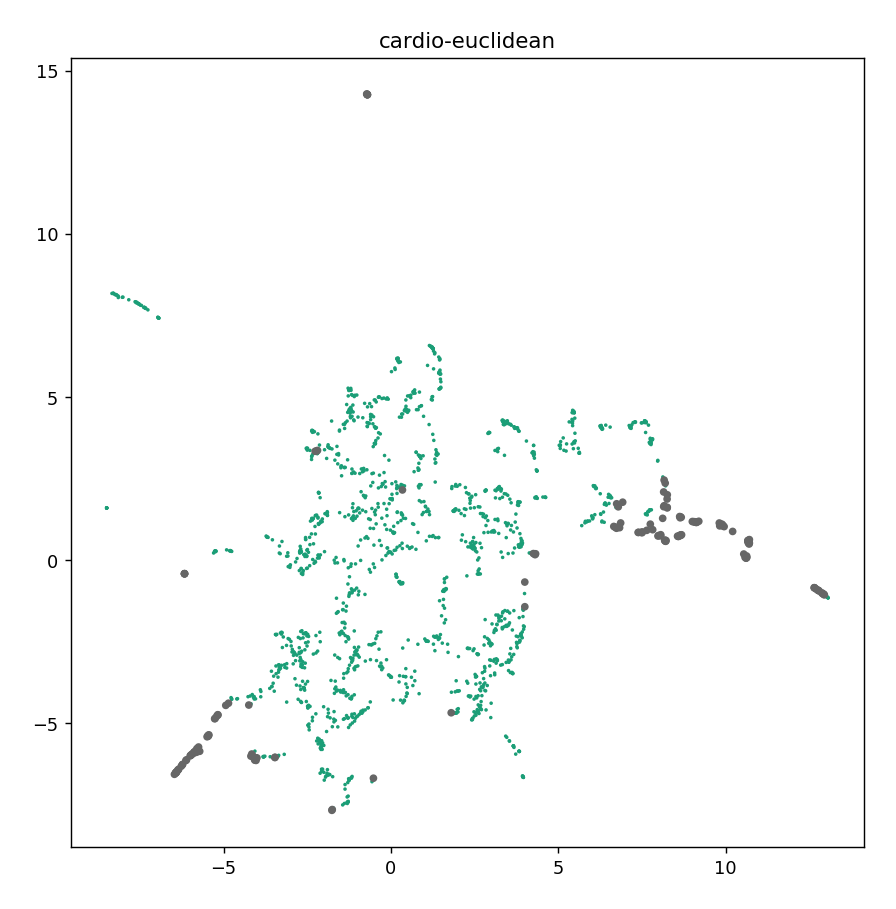
\includegraphics[width=2.3in]{images/umaps/cardio-euclidean-umap2d.png}
   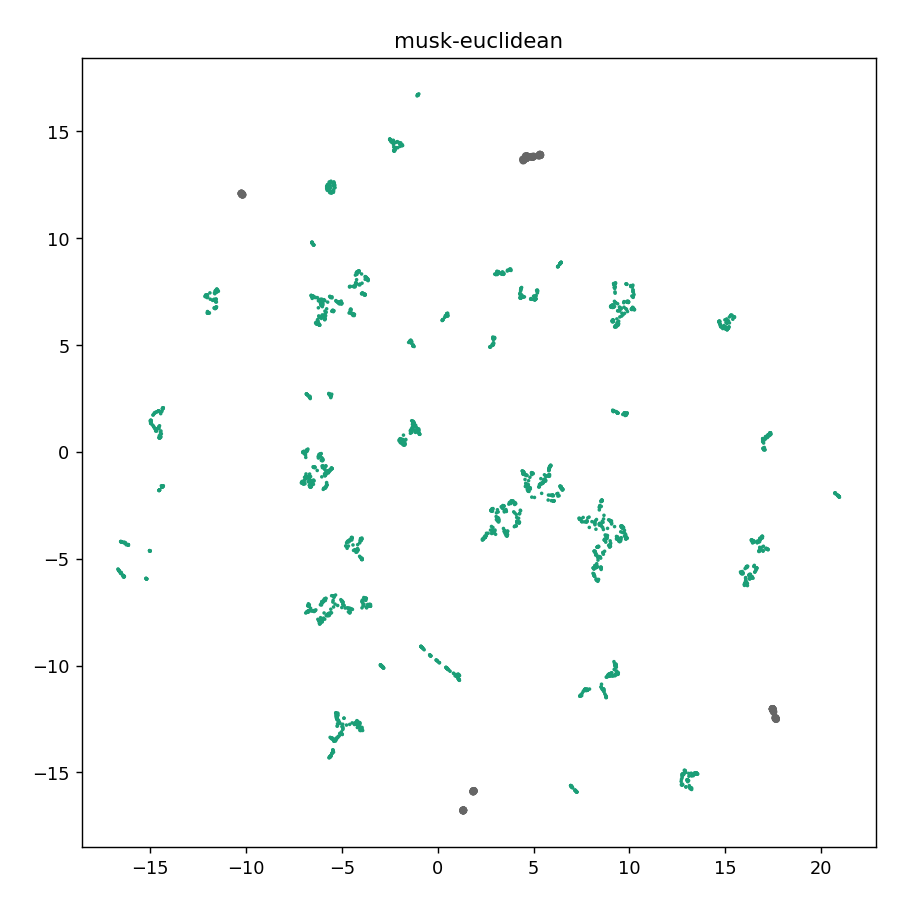
\includegraphics[width=2.3in]{images/umaps/musk-euclidean-umap2d.png}
   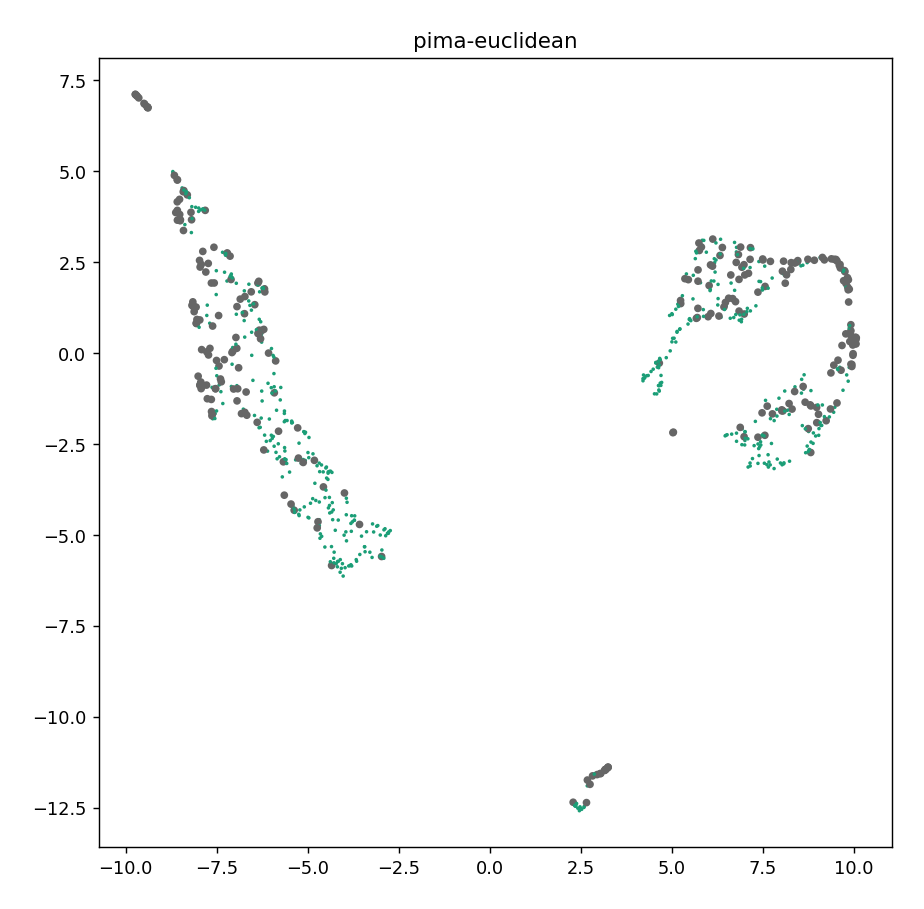
\includegraphics[width=2.3in]{images/umaps/pima-euclidean-umap2d.png}
   \caption{UMAP projections of Cardio (left), Musk (middle), and Pima (right) under Euclidean distance.
   For Cardio, there is a single main component to the manifold, and anomalies tend to be at the edges of that manifold.
   For OptDigits, there are several distinct pieces to the manifold, perhaps corresponding to different digits.
   CHAODA outperforms other approaches on Cardio, while many approaches achieve perfect performance on Musk. On Pima, all approaches fare poorly, and the UMAP projection illustrates that the anomalies cover much of the manifold, including in the interior.}
   \label{fig:conclusions:umap-embeddings-1}
\end{figure*}
